\documentclass[specialist,
               substylefile = ../spbu.rtx,
               subf,href,colorlinks=true, 12pt]{disser}

\usepackage[a4paper,
            mag=1000, includefoot,
            left=3cm, right=1.5cm, top=2cm, bottom=2cm, headsep=1cm, footskip=1cm, twoside]{geometry}
\usepackage[T2A]{fontenc}
\usepackage[utf8]{inputenc}
\usepackage[english,russian]{babel}
\ifpdf\usepackage[outdir=./]{epstopdf}\fi

% Использовать полужирное начертание для векторов
\let\vec=\mathbf

% Включать подсекции в оглавление
\setcounter{tocdepth}{2}

\usepackage[defaultmono]{droidmono}
\usepackage[T2A]{fontenc}
% \usepackage{csquotes}

\usepackage[intlimits]{amsmath}
\usepackage{amsfonts}
\usepackage{amssymb}
\usepackage{amsthm}

\usepackage{algorithm2e}
\usepackage{graphicx}
\graphicspath{ {../media/} }
\usepackage{color}

\usepackage[fixlanguage]{babelbib}
\selectbiblanguage{russian}

% \usepackage{natbib}
% \usepackage[style=numeric]{biblatex}
% \addbibresource{biblio-u.bib}

\usepackage{hyperref}
\newtheorem{theorem}{Теорема}
\newcommand{\ev}{\mathrm{E}}
\newcommand{\vfi}{\varphi}
\newcommand{\veps}{\varepsilon}
\newcommand{\prob}[1]{\mathrm{P}\left(#1\right)}
\newcommand{\R}{\ensuremath{\mathbb{R}}}
\newcommand{\Tau}{\ensuremath{\mathcal{T}}}
\newcommand{\GothB}{\mathfrak{B}}
\newcommand{\norm}[1]{\left\lVert#1\right\rVert}
\newcommand{\Vhat}{\hat{V}}
\newcommand{\Vbar}{\bar{V}}
\newcommand{\vhat}{\hat{v}}
\newcommand{\maxset}[1]{\max\left\lbrace#1\right\rbrace}
\DeclareMathOperator*{\argmax}{arg\,max}
\DeclareMathOperator*{\argmin}{arg\,min}

% \renewcommand\topfraction{0.85}
% \renewcommand\bottomfraction{0.85}
% \renewcommand\textfraction{0.1}
% \renewcommand\floatpagefraction{0.85}
\setlength\parindent{0pt}
\setlength\parskip{0.5em}

\begin{document}

%
% Титульный лист на русском языке
%

% Название организации
\institution{%
    Правительство Российской Федерации \\
    Федеральное государственное бюджетное образовательное учреждение \\
    высшего профессионального образования \\
    «Санкт-Петербургский государственный университет» \\
    Кафедра статистического моделирования
}

\title{Отчет о научно-исследовательской практике}

% Тема
\topic{\normalfont\scshape%
    Имитационная модель американского опциона}

% Автор
\author{Миллер Анастасия Александровна}

% Научный руководитель
\sa       {С.\,М.~Ермаков}
\sastatus {д.\,ф.-м.\,н., профессор}

% Город и год
\city{Санкт-Петербург}
\date{\number\year}

\maketitle
% \newpage\hfill\newpage
\cleardoublepage

\tableofcontents

\intro
    Задачей семестра было исследование поведения оценок \cite{Broadie1997} в дискретном пространстве состояний. \\
    В первой части отчёта приведена формулировка проблемы, как она изложена в \cite{Broadie1997} (с привлечением более удобной нотации из \cite{Kashtanov2015}), и изложен предлагаемый аналог для дискретного пространства состояний. Во второй части отчёта показано, что состоятельность оценки и конечность её дисперсии не меняются при дискретизации пространства состояний. Третья часть содержит расчётные формулы оценки по дискретному пространству состояний для модели Блэка-Шоулса. В четвёртой изложены результаты численного моделирования. 

\chapter{Оценка американского опциона с помощью случайных деревьев: случай непрерывного и дискретного пространств состояний исходного актива}
    Для Американского опциона с функцией выплат $h_t\left(X_t\right)$, где $X_t$ — состояние актива, на который выписан опцион, в момент времени $t\in\left[0;T\right]$, задача оптимального исполнения — это задача о нахождении \begin{equation}\label{eq:optimal_stopping}V = \max_{\tau} \ev h_\tau\left(X_\tau\right).\end{equation}

    При дискретизации \eqref{eq:optimal_stopping} (принятии предположения о том, что опцион может быть исполнен только в некотором конечном числе моментов времени $\left\lbrace t_i\right\rbrace_{i=0}^n \in \left[0;T\right], t_0 = 0, t_n = T$) задача обретает эквивалентную формулировку о нахождении $V_0\left(X_0\right)$ для
    \begin{equation}\label{eq:option-recursive}\begin{aligned}
                V_m\left(x\right) &= h_m\left(x\right), \\
                V_{i-1}\left(x\right) &= \max\left\lbrace h_{i-1}\left(x\right), \ev\left[V_i\left(X_i\right)|X_{i-1}=x\right]\right\rbrace.
    \end{aligned}\end{equation}

    В \cite{Broadie1997} были предложены оценки для $V_0\left(X_0\right)$ (см.~также \cite{Glasserman2004}). Оценка сверху:
    \begin{equation}\label{eq:upper}\begin{aligned}
            \Vhat_m^{j_1 \ldots j_m} &= h_m\left(X_m^{j_1 \ldots j_m}\right), \\
            \Vhat_i^{j_1 \ldots j_i} &= \max \left\lbrace h_i \left( X_i^{j_1 \ldots j_i} \right), \frac{1}{b} \sum_{j = 1}^b \Vhat_{i+1}^{j_1 \ldots j_i j}\right\rbrace.
    \end{aligned}\end{equation}

    Оценка снизу:
    \begin{equation}\label{eq:lower}\begin{aligned}
        \vhat_m^{j_1 j_2 \cdots j_m} &= h\left( X_m^{j_1 j_2 \cdots j_m}\right), \\
        \vhat_{ik}^{j_1 j_2 \cdots j_i} &= \left\lbrace\begin{array}{l l}
            h\left( X_i^{j_1 j_2 \cdots j_i}\right), & \, \text{если } \frac{1}{b-1}\sum_{j=1, j\not= k}^b \vhat_{i+1}^{j_1 j_2 \cdots j_i j} \leq h\left(X_i^{j_1 j_2 \cdots j_i}\right), \\
            \vhat_{i+1}^{j_1 j_2 \cdots j_i k}, & \, \text{иначе,}
            \end{array}\right. \\
        \vhat_i^{j_1 j_2 \cdots j_i} &= \frac{1}{b}\sum_{k=1}^b \vhat_{ik}^{j_1 j_2 \cdots j_i}.
    \end{aligned}\end{equation}

    Здесь предполагается, что $X_t$ -- Марковский случайный процесс, последовательность $\left\lbrace X_k^{j_1\cdots j_k}\right\rbrace_{k=1}^m$ -- реализация траектории $X_t$. Подробно процесс генерации случайного дерева $\left\lbrace X_k^{j_1\cdots j_k}\right\rbrace$ описан в \cite{Broadie1997}.

    В дальнейшем мы ограничимся только рассмотрением оценки сверху, как более простой по построению. 

    В \cite{Broadie1997} доказано, что 
    \begin{theorem}
        $\exists p' > 1: \forall\: t \in \left[0; T\right]\: \ev \left\vert h_t\left(X_t\right)\right\vert ^{p'} < \infty \implies$ \\
        $\Vhat_0(X_0)$ сходится к $V_0(X_0)$ в $L^p$ $\forall\: 0 < p < p'$ при $b \to \infty$.
    \end{theorem}
    То есть, в частности, если функция выплат имеет конечный третий момент, то оценка $\Vhat_0(X_0)$ имеет конечную дисперсию.

    При этом понятно, что при увеличении $b \to\infty$ время, требуемое для подсчёта $\Vhat_0(X_0)$, растёт как $O\left(b^m\right)$. Одним из способов ограничить этот рост, не меняя принципиально структуру оценки, является дискретизация пространства состояний: если на $k$-м шаге $S_k \in \left\lbrace S_k^i\right\rbrace_{i=1}^N$, то количество различных вершин дерева на $k$-м шаге, равное в схеме \eqref{eq:upper} $b^k$, не может превосходить $N$. Таким образом, мы получаем временные затраты порядка, не превосходящего $O(Nm)$.

    Рассмотрим подробнее процесс перехода из непрерывного пространства состояний в дискретное. 

    Пусть состояние актива, на который выписан опцион, представимо в виде Марковского процесса $X_n$ с началом в точке $X_0$ и переходными плотностями $p_n(X_{n-1}, X_n)$. Тогда можно построить процесс с дискретным носителем $\bar X_n$, определив множество его допустимых состояний $X_n$ как множество квантилей распределения с плотностью $p_n\left(X_0, \cdot\right)$: $S_n^i$ -- это $\frac{2i - 1}{N}$-квантиль распределения с плотностью $p_n\left(X_0, \cdot\right)$, $i\in 1\mathbin{:} N$. Заметим, что очевидным образом такая операция осуществима только в случае $X_t\in\R$, в больших размерностях понятие квантиля требует уточнения.

    В процессе построения дерева мы генерировали $X_k^{j_1\cdots j_k}$ с плотностью $p_k\left(X_{k-1}^{j_1\cdots j_{k-1}}, \cdot \right)$. Теперь носитель распределения для $\bar X_k^{j_1\cdots j_k}$ --- только лишь $\left\lbrace S_k^i\right\rbrace$. Будем дискретизировать распределение естественным образом:
    \[
        \prob{\bar X_k^{j_1\cdots j_k} = S_k^i} = \int_{\frac{1}{2}\left(S_k^{i-1} + S_k^{i}\right)}^{\frac{1}{2}\left(S_k^{i} + S_k^{i+1}\right)} p_k\left(X_{k-1}^{j_1\cdots j_{k-1}}, u\right) du = p_k^i.
    \]

    При этом если для некоторого набора $j_1',\cdots j_k'$ существует $\bar X_k^{j_1',\cdots j_k'} = \bar X_k^{j_1\cdots j_k}$, то мы считаем эти точки совпадающими и далее генерируем из них только один набор состояний на шаге $k+1$. Тем самым мы теряем независимость траекторий $\left\lbrace \bar X_k^{j_1\cdots j_k}\right\rbrace_{k=1}^m$, но при $N \to \infty$ вероятность совпадения уменьшается и траектории становятся всё более независимыми.

    Оценка \eqref{eq:upper} остаётся неизменной:

    \begin{equation}\label{eq:discrete}\begin{aligned}
            \Vbar_m^{j_1 \ldots j_m} &= h_m\left(\bar X_m^{j_1 \ldots j_m}\right), \\
            \Vbar_i^{j_1 \ldots j_i} &= \max \left\lbrace h_i \left( \bar X_i^{j_1 \ldots j_i} \right), \frac{1}{b} \sum_{j = 1}^b \Vbar_{i+1}^{j_1 \ldots j_i j}\right\rbrace.
    \end{aligned}\end{equation}
    Заметим, что в сумме $\sum_{j = 1}^b \Vbar_{i+1}^{j_1 \ldots j_i j}$, в отличие от оценки $\Vhat$, слагаемые могут совпадать с положительной вероятностью.

\chapter{Моменты оценки по дискретному пространству состояний}
    
    Покажем теперь, что $\Vbar_0(X_0)$ является состоятельной оценкой $V_0(X_0)$. Заметим, что и $\Vbar$, и $\Vhat$ являются одной и той же детерминированной функцией он стохастического дерева $\left\lbrace X_k^{j_1\cdots j_k}\right\rbrace$. В \cite{Broadie1997} доказано, что при $b \to \infty$ оценка $\Vhat_0(X_0, b)\to V_0(X_0)$. Следовательно, остаётся доказать лишь то, что при $N\to\infty$ деревья $\left\lbrace X_k^{j_1\cdots j_k}\right\rbrace$ и $\left\lbrace \bar X_k^{j_1\cdots j_k}\right\rbrace$ в некотором смысле совпадают.

    Напомним, что процесс $\bar X_n$ задаётся следующим образом:  
    $$\forall\:i\in 1\mathbin : N\:\: \exists\: p_n^i = \int_{\frac{1}{2}\left(S_n^{i-1} + S_n^{i}\right)}^{\frac{1}{2}\left(S_n^{i} + S_n^{i+1}\right)} p_n\left(\bar X_{n-1}, u\right) du,$$ 
    где граничные точки $S_n^0 = -\infty, S_n^{N+1} = \infty$, а $S_n^i$ -- это $\frac{2i-1}{N}$-квантиль распределения с плотностью $p_n\left(X_0, \cdot\right)$; тогда
    $$\mathcal P\left(\bar X_n\middle\vert \bar X_{n-1}\right) = \mathcal P \begin{pmatrix} S_n^i\\ p_n^i \end{pmatrix}.$$

    \begin{theorem}
        Для любого непрерывного семейства плотностей $p_n\left(x, y\right)$ и случайных процессов $X_n \sim \mathcal P_{p_n\left(X_{n-1}, \cdot\right)}$, $\bar X_n$ при $N\to\infty$ распределение процесса $\bar X_n$ сходится к распределению процесса $X_n$.
    \end{theorem}
    \begin{proof} 
        Так как оба процесса Марковские, достаточно доказать, что 
        $$\mathcal P\left(\bar X_n\middle\vert \bar X_{n-1} = C\right) \to \mathcal P\left(X_n\middle\vert X_{n-1} = C\right).$$

        По построению для любого $\veps > 0, \left( a; b\right) \subset \R \: \exists N, i, j \in 1\mathbin : N$ такие, что 
        $$ \begin{cases}
        S_n^{i-1} < a \leq S_n^i \leq S_n^j \leq b < S_n^{j+1}, \\
        \left\vert\int_{S_n^{i-1}}^a p_n\left(\bar X_{n-1}, u\right) du\right\vert < \veps, \\
        \left\vert\int_{b}^{S_n^{j+1}} p_n\left(\bar X_{n-1}, u\right) du \right\vert< \veps.
        \end{cases} $$
        (то есть можно выбрать $N$ такое, чтобы квантили достаточно плотно окружали границы отрезка). Тогда 
        \begin{align*}
            &\left\vert 
                \prob{\bar X_n \in \left( a; b\right)} - 
                \prob{X_n \in \left( a; b\right)} 
            \right\vert = \\ &= 
            \left\vert 
                \int_{\frac{1}{2}\left(S_n^{i-1} + S_n^{i}\right)}^{\frac{1}{2}\left(S_n^{j} + S_n^{j+1}\right)} p_n\left(C, u\right) du - \int_a^b p_n\left(C, u\right) du 
            \right\vert \leq \\ &\leq 
            \left\vert 
                \int_{S_n^{i-1}}^{a} p_n\left(C, u\right) du + \int_{b}^{S_n^{j+1}} p_n\left(C, u\right) du 
            \right\vert \leq 2\veps
        \end{align*}

        То есть при $N\to\infty$ $\mathcal P\left(\bar X_n\middle\vert \bar X_{n-1} = C\right) \to \mathcal P\left(X_n\middle\vert X_{n-1} = C\right)$.
    \end{proof}

    Следовательно, все предельные выводы, верные для $\Vhat_0(X_0)$ верны и для $\Vbar_0(X_0)$ при дополнительном устремлении $N\to\infty$. В частности, если функция выплат имеет конечный третий момент, то оценка $\Vbar_0(X_0)$ состоятельна и имеет конечную дисперсию.

\chapter{Расчётные формулы для модели Блэка-Шоулса}
    В модели Блэка-Шоулса состояние актива $X_t$ подчиняется дифференциальному уравнению $$\frac{d X_t}{X_t} = \left(r - \delta\right) dt + \sigma d w_t,$$ где $w_t$ -- винеровский процесс. Для сокращения записи обозначим также $\mu = r - \delta$, ширину отрезка дискретизации по времени $T / m = \Delta t$. Тогда $\forall\: 0 \leq k \leq n \leq m$ $$X_n = X_k\exp\left(\left(\mu - \frac{\sigma^2}{2}\right)\Delta t\left(n-k\right) + \sigma\Delta t \left(n-k\right) \veps\right),$$ где $\veps\sim \mathcal N(0, 1)$. Величина $X_n / X_k \sim \ln N\left(\left(\mu - \frac{\sigma^2}{2}\right)\Delta t\left(n - k\right), \sigma^2 \Delta t\left(n - k\right)\right)$. Следовательно, квантили $S_n^i$ могут быть вычислены через соответствующие квантили стандартного нормального распределения $\veps_i$ как
    \begin{equation}\label{eq:bs_quantile}
        S_n^i = X_0\exp\left(\left(\mu - \frac{\sigma^2}{2}\right)n\Delta t + \sigma n\sqrt{\Delta t} \veps_i\right).
    \end{equation}

    Вероятности $p_n^i$ аналогичным образом пересчитываются через функцию распределения нормального распределения:
    \begin{equation}\label{eq:bs_probabilities}
    \begin{aligned}
        p_n^i &= \prob{\frac{1}{2}\left(S_k^{i-1} + S_k^i\right) < X_k < \frac{1}{2}\left(S_k^{i} + S_k^{i+1}\right)\middle\vert X_{k-1}} = \\
        &=\prob{\ln\frac{\frac{1}{2}\left(S_k^{i-1} + S_k^i\right)}{X_{k-1}} < \ln\frac{X_k}{X_{k-1}} < \ln\frac{\frac{1}{2}\left(S_k^{i} + S_k^{i+1}\right)}{X_{k-1}}} = \\
        &= \Phi_{\left(\mu - \frac{\sigma^2}{2}\right)\Delta t\left(n - k\right), \sigma^2 \Delta t\left(n - k\right)}\left(\ln\frac{\frac{1}{2}\left(S_k^{i} + S_k^{i+1}\right)}{X_{k-1}}\right) - \\ &\quad-\Phi_{\left(\mu - \frac{\sigma^2}{2}\right)\Delta t\left(n - k\right), \sigma^2 \Delta t\left(n - k\right)}\left(\ln\frac{\frac{1}{2}\left(S_k^{i-1} + S_k^{i}\right)}{X_{k-1}}\right).
    \end{aligned}
    \end{equation}

    Как видно из выражений \eqref{eq:bs_quantile} и \eqref{eq:bs_probabilities}, самой вычислительно сложной операцией в подсчёте $\Vbar_0(X_0)$ будет вычисление функции распределения $\Phi$, а все вычисления интегралов неизвестной заранее плотности можно обойти.
    % Тогда переходные плотности будут иметь вид
    % \[
    %     p_n\left(S, x\right) = \frac{1}{x\sqrt{2\pi\sigma^2 \Delta t}}\exp\left(-\frac{\left(\ln\frac{x}{S} - \left(\mu - \frac{\sigma^2}{2}\right)\Delta t\right)^2}{2\sigma^2\Delta t}\right).
    % \]




\chapter{Численные результаты}
    Предложенный алгоритм был реализован для подсчёта примера, опубликованного в статье \cite{Broadie1997}. Ниже приведены результаты моделирования для различных параметров опциона и различных частот дискретизации пространства состояний.
    
    Оценивалась цена Бермудского опциона с четырьмя моментами исполнения, в моменты $t \in \left\lbrace 0, T/3, 2T/3, T\right\rbrace$ (так как для неё возможно получить референсные значения методом стохастического дерева без дискретизации пространства параметров). Результаты представлены на рис. \ref{fig:value}. Видно, что в одномерном случае дискретизация пространства параметров незначительно увеличивает дисперсию при существенном выигрыше в трудоёмкости. Трудоёмкость, измеренная в количестве элементарных операций, представлена на рис. \ref{fig:complexity}: для дискретизованного пространства состояний трудоёмкость естественным образом ограничена размером пространства состояний, тогда как для непрерывного пространства состояний имеем экспоненциальный рост трудоёмкости при увеличении числа ветвей в дереве $b$.
    \begin{figure}[h]
    		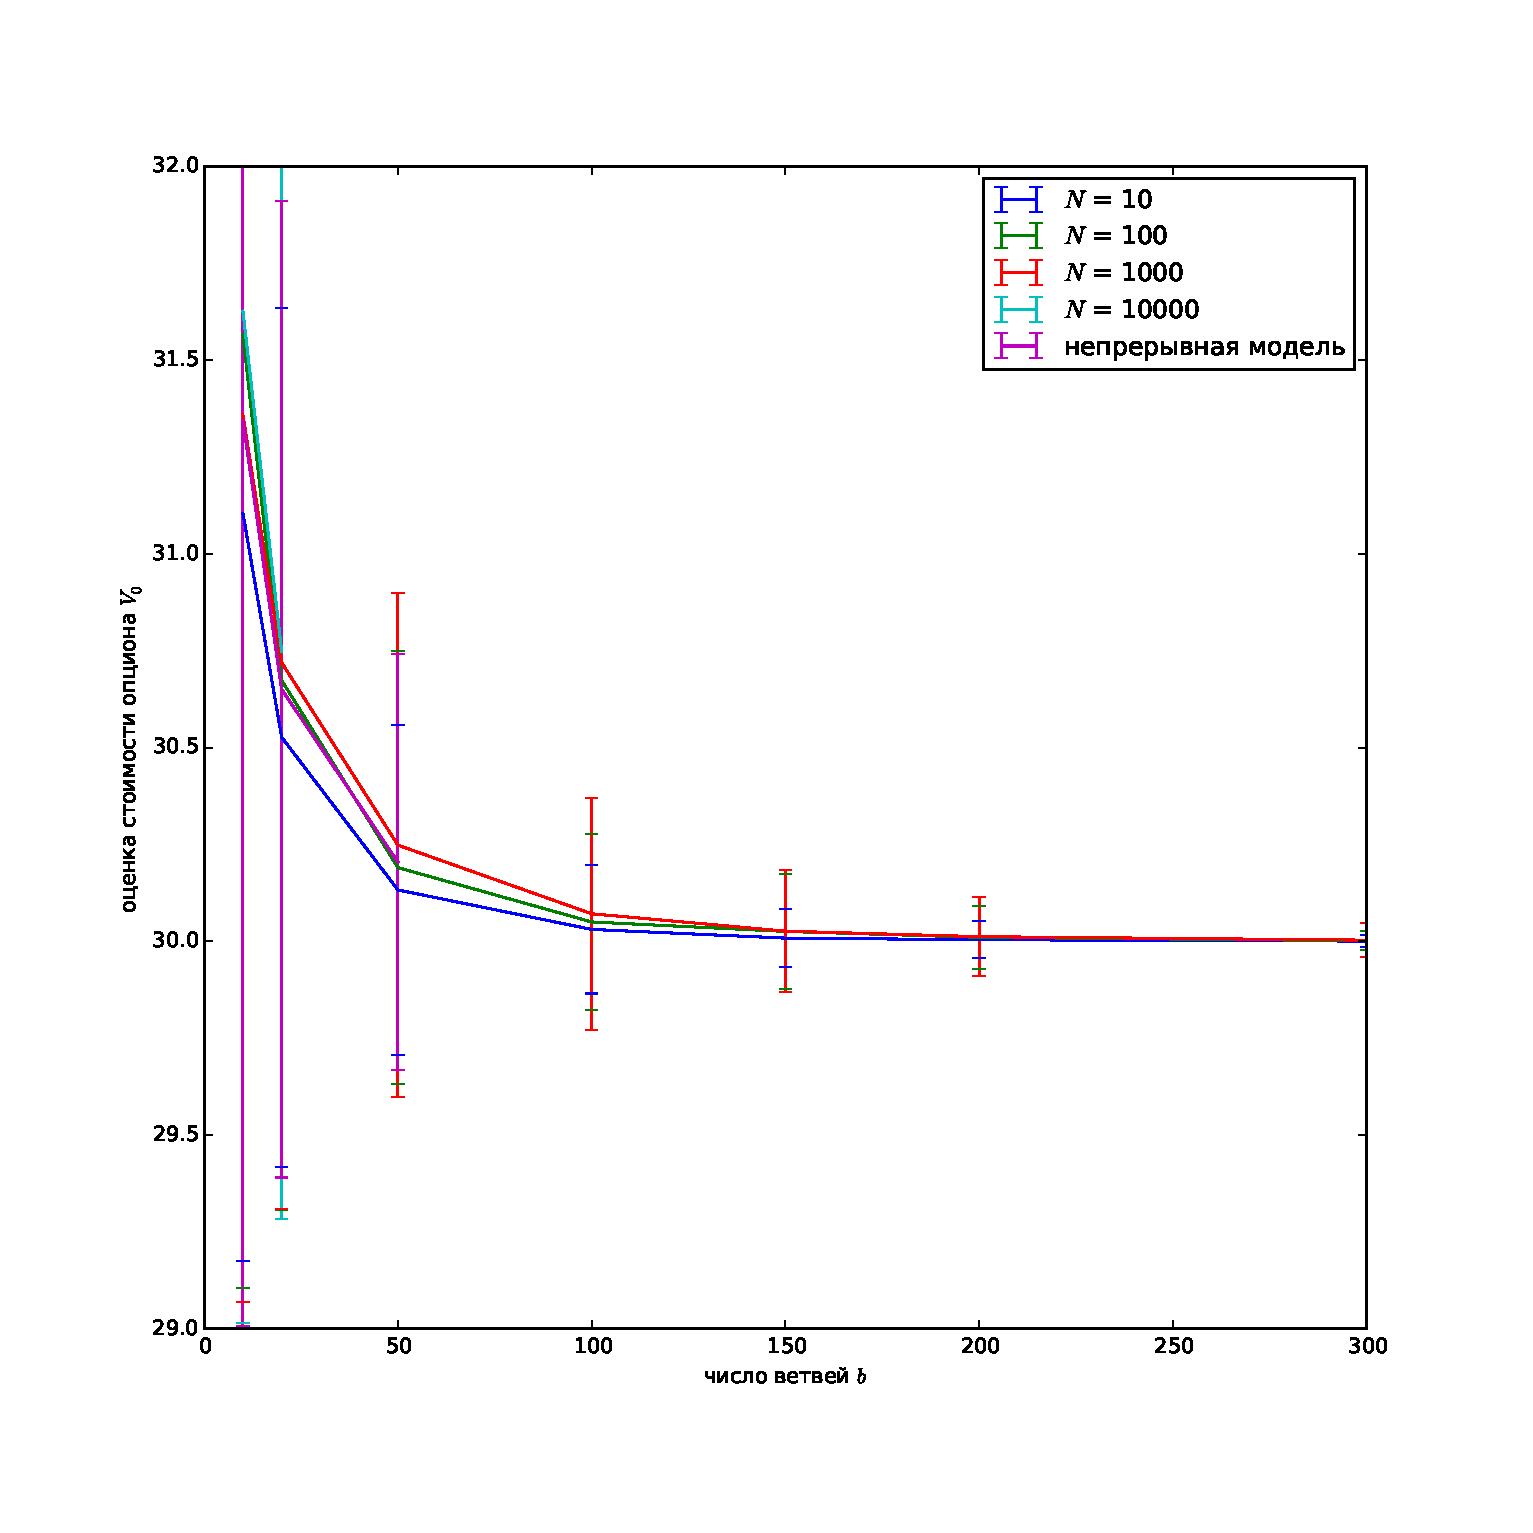
\includegraphics[width=\textwidth]{130}
    		\caption{Значения и ошибки оценки стоимости Бермудского опциона с 4 моментами исполнения при использовании разных методов оценки}
    		Параметры опциона: $r = 5\%, \delta = 10\%, \sigma = 20\%$. Начальная цена актива $S_0 = 130$, цена страйк $K = 100$, опцион выписан на $T=1$ год.
    		\label{fig:value}
	\end{figure}
    \begin{figure}[h]
    		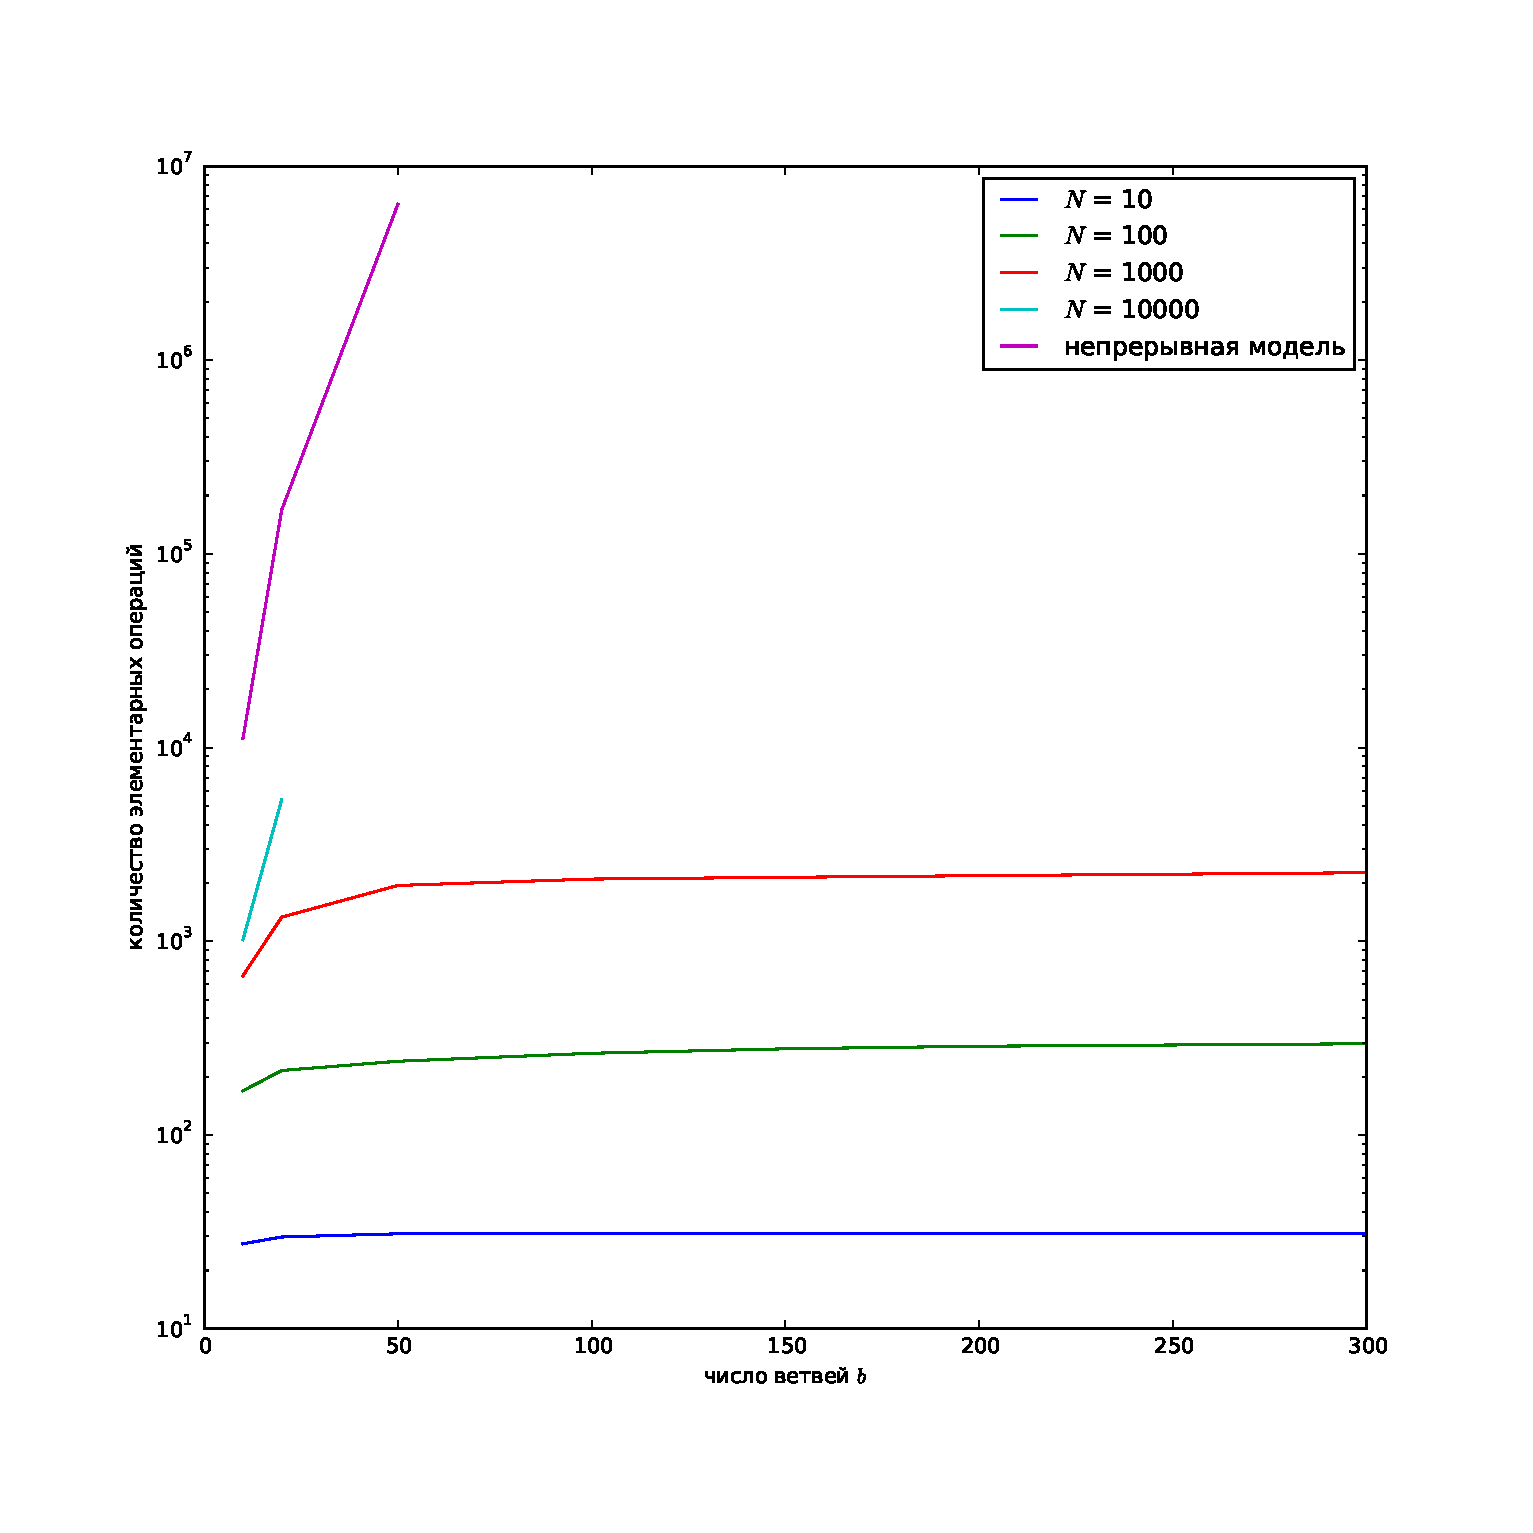
\includegraphics[width=\textwidth]{complexity_130}
    		\caption{Количество элементарных операций для подсчёта оценки стоимости опциона при использовании разных методов подсчёта}
    		\label{fig:complexity}
	\end{figure}

\conclusion
    В этом семестре мною была формализована оценка Американского опциона методом случайных деревьев по дискретному пространству состояний, доказаны состоятельность этой оценки и конечность её дисперсии. Ближайшими планами являются представление вычислительных результатов, численная оценка дисперсии и её теоретическое подтверждение.
    

\bibliographystyle{ugost2008}
\bibliography{../biblio-u}
\end{document}